% These are the lecture notes for my CSCI360 course SPRING 2017
% at John Jay College of Criminal Justice. They are based largely on
% Schneier's Applied Cryptography.

% Feel free to edit these slides and use them for your own courses.
% HOWEVER DO NOT REMOVE THESE LINES!
% Email me at: awood [at] jjay.cuny.edu
% or at: awood [at] gradcenter.cuny.edu


\documentclass{beamer}

\usepackage{tikz}
\usetikzlibrary{calc}

\usepackage{forest}
\usepackage{verbatim}
\usepackage{color}
\usepackage{amsmath}


\setbeamertemplate{footline}[frame number]
\setbeamertemplate{navigation symbols}{} 

\newtheorem{thm}{Theorem}[section]
\newtheorem{lem}{Lemma}
\newtheorem{cl}{Claim}
\newtheorem{cor}{Corollary}[section]
\newtheorem{conj}{Conjecture}
\newtheorem{quest}{Question}
\newtheorem{defn}{Definition}[section]
\newtheorem{obs}{Observation}[section]
\newtheorem{exam}{Example}

\newcommand{\im}{\operatorname{im}}
\newcommand{\id}{\operatorname{id}}
\newcommand{\interior}{\operatorname{int}}
\newcommand{\bdry}{\operatorname{bdry}}
\newcommand{\<}{\langle}
\renewcommand{\>}{\rangle}
\newcommand{\Gab}{(G_\phi)^{ab}} 
\newcommand{\phibar}{\bar{\phi}}
\newcommand{\Z}{\mathbb{Z}}
\newcommand{\N}{\mathbb{N}}
\newcommand{\Q}{\mathbb{Q}}
\newcommand{\R}{\mathbb{R}}
\newcommand{\C}{\mathbb{C}}
\newcommand{\A}{\mathcal{A}}
\newcommand{\OO}{\mathcal{O}}
\newcommand{\UU}{\mathcal{U}}
\newcommand{\power}{2^{\{P_1, \cdots , P_n\}}}
\newcommand{\bp}{\begin{problem}}
\newcommand{\ep}{\end{problem}}
\newcommand{\ba}{\begin{answer}}
\newcommand{\ea}{\end{answer}}
\newcommand{\ds}{\displaystyle}
\newcommand{\ben}{\renewcommand{\theenumi}{\alph{enumi}}
\renewcommand{\labelenumi}{(\theenumi)}\begin{enumerate}}
\newcommand{\een}{\end{enumerate}}
\newcommand{\Hess}{\operatorname{Hessian}}
\newcommand{\Aut}{\mathrm{Aut}}
\newcommand{\Inn}{\mathrm{Inn}}
\newcommand{\Out}{\mathrm{Out}}
\newcommand{\End}{\mathrm{End}}


\mode<presentation>
{
%  \usetheme{default}
  \setbeamercovered{invisible}
}


\usepackage[english]{babel}
\usepackage[latin1]{inputenc}
\usepackage{times}
\usepackage[T1]{fontenc}
\usepackage{stmaryrd}

%\usetheme{default}
%\usetheme{AnnArbor}
%\usetheme{Antibes}
%\usetheme{Bergen}
%\usetheme{Berkeley}
%\usetheme{Berlin}
%\usetheme{Boadilla}
%\usetheme{CambridgeUS}
%\usetheme{Copenhagen}
%\usetheme{Darmstadt}
%\usetheme{Dresden}
%\usetheme{Frankfurt}
%\usetheme{Goettingen}
%\usetheme{Hannover}
%\usetheme{Ilmenau}
%\usetheme{JuanLesPins}
%\usetheme{Luebeck}
%\usetheme{Madrid}
%\usetheme{Malmoe}
%\usetheme{Marburg}
%\usetheme{Montpellier}
%\usetheme{PaloAlto}
%\usetheme{Pittsburgh}
%\usetheme{Rochester}
\usetheme{Singapore}
%\usetheme{Szeged}
%\usetheme{Warsaw}

%\usecolortheme{default}
%\usecolortheme{albatross}
\usecolortheme{beaver}
%\usecolortheme{beetle}
%\usecolortheme{crane}
%\usecolortheme{dolphin}
%\usecolortheme{dove} % grey, white, yellow
%\usecolortheme{fly} %grey, yellow
%\usecolortheme{lily} %white, yellow, blue
%\usecolortheme{orchid}
%\usecolortheme{rose}
%\usecolortheme{seagull}
%\usecolortheme{seahorse}
%\usecolortheme{whale}
%\usecolortheme{wolverine}

% Title page

\title[OOP]{Cryptographic Attack Models}

\subtitle{Based on \emph{Cryptography Engineering} sections 2.6, 2.7 \\ By Ferguson, Schnier, and Kohno}

\author
{Lecture notes of Alexander Wood \\ \scriptsize \href{mailto:awood@jjay.cuny.edu}{awood@jjay.cuny.edu}}
\institute[JJay]{John Jay College of Criminal Justice}  

\date{}

\begin{document}

% Remove 'figure' text from figure captions 
\setbeamertemplate{caption}{\raggedright\insertcaption\par}

\begin{frame}
  \titlepage
\end{frame}


\section{Cryptanalysis}



\begin{frame}
\frametitle{Kerckhoffs' Principle}

Recall \textbf{Kerckhoffs' Principle}, formulated by the Dutch mathematician in the 1880s. \newline

This principle states that \emph{we should be able to publish all of the information about how the cryptosystem works without compromising its security.}
\end{frame}

\begin{frame}
\frametitle{Cryptanalytic Attack Models}

First we will go over attack models which aim to recover either the \emph{plaintext} or the \textbf{decryption key}.

\begin{itemize}
\item Ciphertext-Only Model
\item Known-Plaintext Model
\item Chosen-Plaintext Model
\item Adaptive-Chosen-Plaintext Model
\item Chosen-Ciphertext Model
\end{itemize}
\end{frame}


\begin{frame}
\frametitle{Ciphertext-Only Model}

This model is the most basic model, and is what people usually mean when they discuss breaking encryption. In this model, Eve is eavesdropping on communication between Alice and Bob, and all she sees as the attacker is the ciphertexts.

\begin{itemize}
\item \emph{Given}: Ciphertexts $C_1$, $C_2$, $\dots, C_k$
\item \emph{Deduce:} $M_1$, $M_2, \dots, M_k$ or $Enc()$.
\end{itemize}

She attempts to use properties of these plaintexts to deduce either the contents of the messages, the keys, or both. 
\end{frame}


\begin{frame}
\frametitle{Ciphertext-Only Model}

Eve tries to determine they key(s) or the plaintext(s) by analyzing intercepted ciphertexts.

\begin{figure}
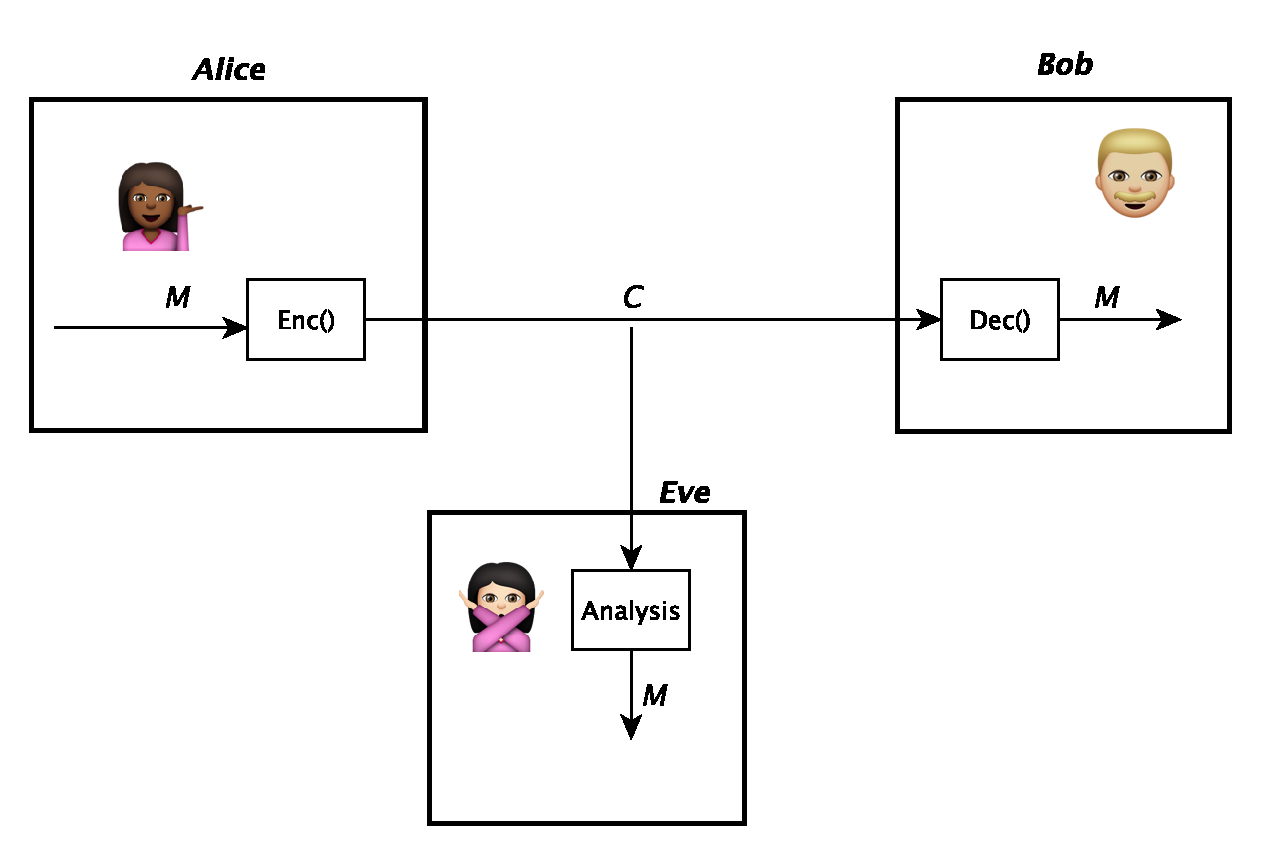
\includegraphics[scale=.4]{IMG/attack1.pdf}
\end{figure}
\end{frame}


\begin{frame}
\frametitle{Ciphertext-Only Model}

We saw how to break several encryption systems using the ciphertext-only model.
\begin{itemize}
\item We broke the \textbf{Caesar Shift} using a brute-force attack in the ciphertext-only model.
\item We broke the \textbf{substitution cipher} using a frequency analysis attack in the ciphertext-only model. 
\end{itemize}
\end{frame}


\begin{frame}
\frametitle{Ciphertext-Only Model}

This is generally considered the most difficult type of attack because the attacker has the least amount of information to work with. \newline

Often, we are in situations where the attacker has access to more information than just the ciphertexts. 
\end{frame}


\begin{frame}
\frametitle{Known-Plaintext Model}

A \textbf{known-plaintext attack} is carried out when Eve knows both the plaintext and the ciphertext. 

\begin{itemize}
\item \emph{Given:} Plaintexts and their associated ciphertexts
\item \emph{Deduce:} Decryption key and/or a method of deducing plaintexts from ciphertexts

Now, Eve not only as access to the ciphertext of several messages, but also their corresponding plaintexts. She must deduce the key(s) to the algorithm, or a method of obtaining the plaintexts from ciphertexts.
\end{itemize}
\end{frame}


\begin{frame}
\frametitle{Known-Plaintext Model}

Why do we consider this model? What we need to ask is, when could Eve have access to plaintext?\newline

Occasionally there are messages which are easy to predict. Consider the Bombe machine's attack on the Enigma in WWII. The plaintexts ``Wetterbericht'' (weather report) and ``Heil Hitler'' were essentially guaranteed to appear in some messages. The Bombe machine carried out a \textbf{known-plaintext attack}. 
\end{frame}

\begin{frame}
\frametitle{Known-Plaintext Model}

Eve uses the knowledge of some plaintext-ciphertext pairs in order to deduce the key, which she can use to decrypt new ciphertexts.

\begin{figure}
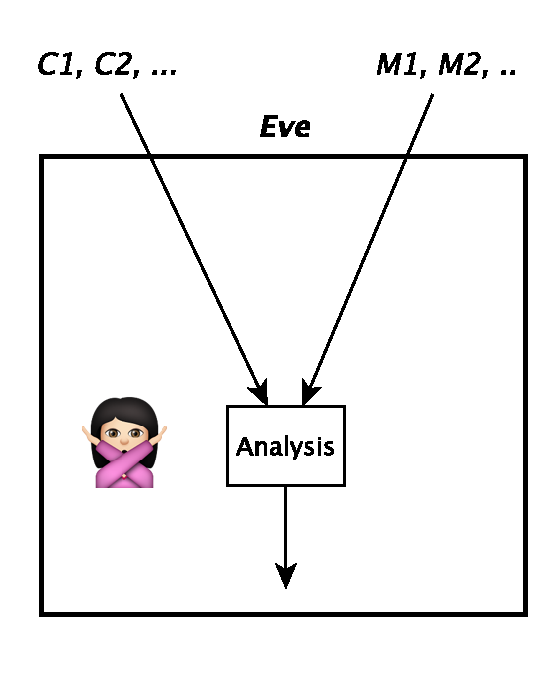
\includegraphics[scale=.4]{IMG/attack2.pdf}
\end{figure}
\end{frame}


\begin{frame}
\frametitle{Chosen-Plaintext Model}

This is a more powerful model. Eve has access to plaintexts and their corresponding ciphertexts, as before. However in a chosen-plaintext attack, Eve gets to choose which plaintexts to encrypt! \newline
This is a relevant attack which any good cryptosystem should be able to withstand. For example, say Eve sends Alice and email which she knows she will encrypt and forward to Bob. 
\end{frame}

\begin{frame}
\frametitle{Chosen-Plaintext Model: The Game}

Cryptographer Victor Shoup has presented models for security proofs as \textbf{sequences of games}. In the Chosen-Plaintext Game,
\begin{enumerate}
\item Eve chooses plaintext messages $M_1, M_2,\dots, M_n$ to encrypt.
\item Eve is given access to an \textbf{encryption oracle}, which returns to her the corresponding ciphertexts $C_1, C_2, \dots, C_n$. 
\item Eve deduces the decryption key using a chosen-plaintext attack.
\end{enumerate}
\end{frame}

\begin{frame}
\frametitle{Chosen Plaintext Model}
\begin{columns}
\column{0.38\linewidth}
\centering
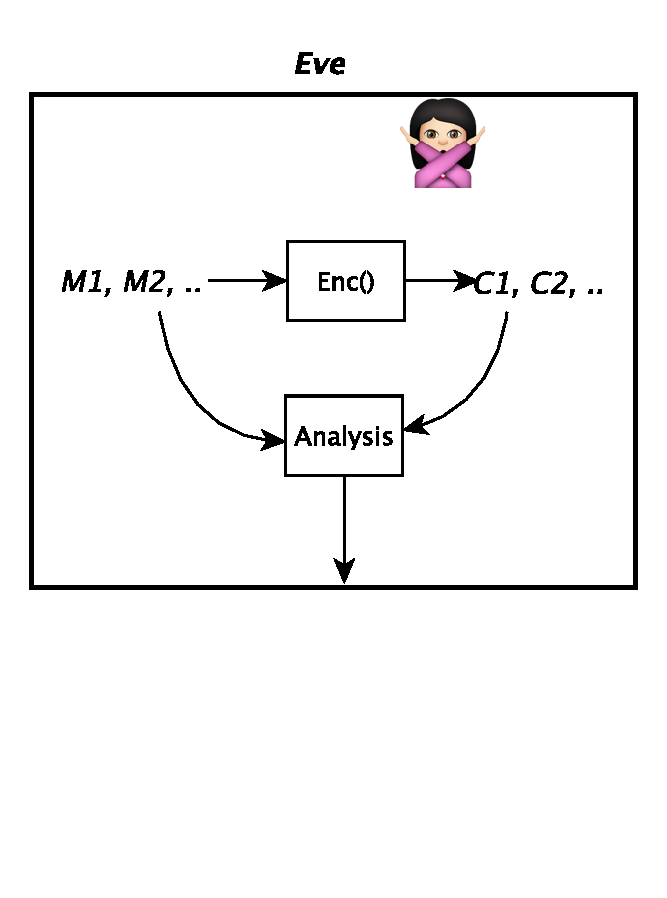
\includegraphics[scale=.5]{IMG/attack2half.pdf}
\column{0.3\linewidth}
Eve chooses which plaintexts to encrypt. 
\end{columns} 
\end{frame}


\begin{frame}
\frametitle{Chosen-Plaintext Model: Private Key}

In the private key model, a known-plaintext attack is less common because the only information Eve can eavesdrop on is the ciphertexts. She does not have any method of encrypting messages herself.
\begin{figure}
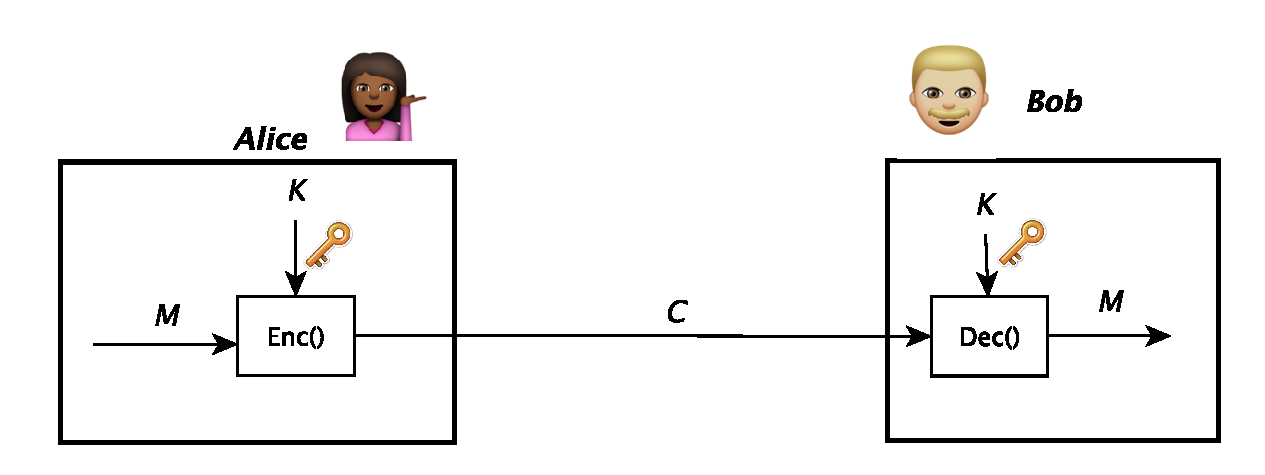
\includegraphics[scale=.5]{IMG/private_key.pdf}
\end{figure}
\end{frame}


\begin{frame}
\frametitle{Chosen Plaintext Model: Public Key Cryptosystems}

What happens if a public-key cryptosystem is vulnerable to a chosen-plaintext attack? \newline

If the encryption key is a \textbf{public key}, then vulnerability to a chosen-plaintext attack comprimises the security of the cryptosystem. Eve can access the plaintext-ciphertext pair of any plaintext she chooses. 
\end{frame}




\begin{frame}
\frametitle{Adaptive-Chosen-Plaintext Model}

\begin{columns}
\column{0.38\linewidth}
\centering
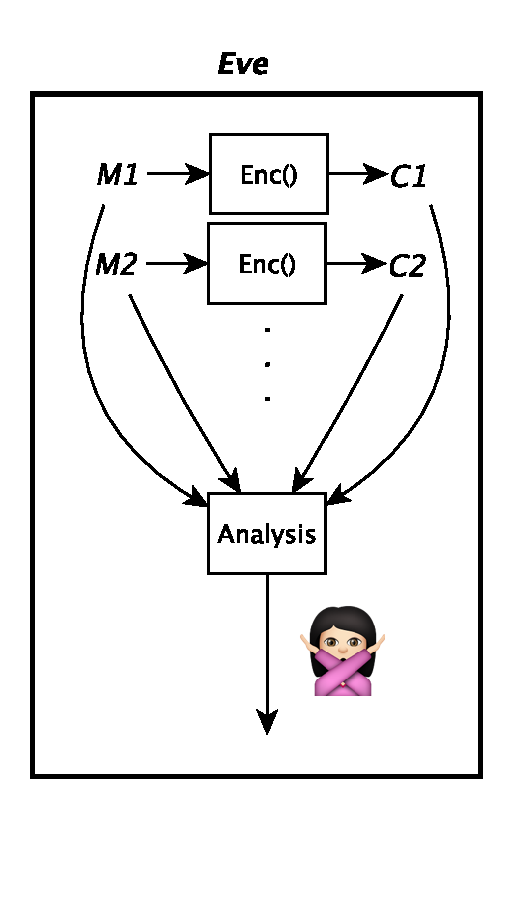
\includegraphics[scale=.5]{IMG/attack3.pdf}
\column{.58\linewidth}
This is similar to the previous model. However, before, Eve had to choose all of the plaintexts she would like to encrypt up front. Now, Eve can adapt the plaintexts she encrypts based off of previous encryptions. \newline
\end{columns} 
\end{frame}


\begin{frame}
\frametitle{Adaptive-Chosen-Plaintext Model: The Game}

\begin{enumerate}
\item For as long as Eve chooses, she carries out the following:
	\begin{enumerate}
	\item Eve chooses a message $M$.
	\item Eve receives its encryption $C$.
	\item Eve analyzes the plaintext-ciphertext pairs she has collected. She uses this knowledge to prepare her next message. 
	\end{enumerate}
\item Eve deduces the decryption key.
\end{enumerate}
\end{frame}

\begin{frame}
\frametitle{Adaptive-Chosen-Plaintext Model: Public Key}
\small
In the public-key model it is sometimes imperative that the cryptosystem can withstand an adaptive chosen plaintext attack.
\begin{figure}
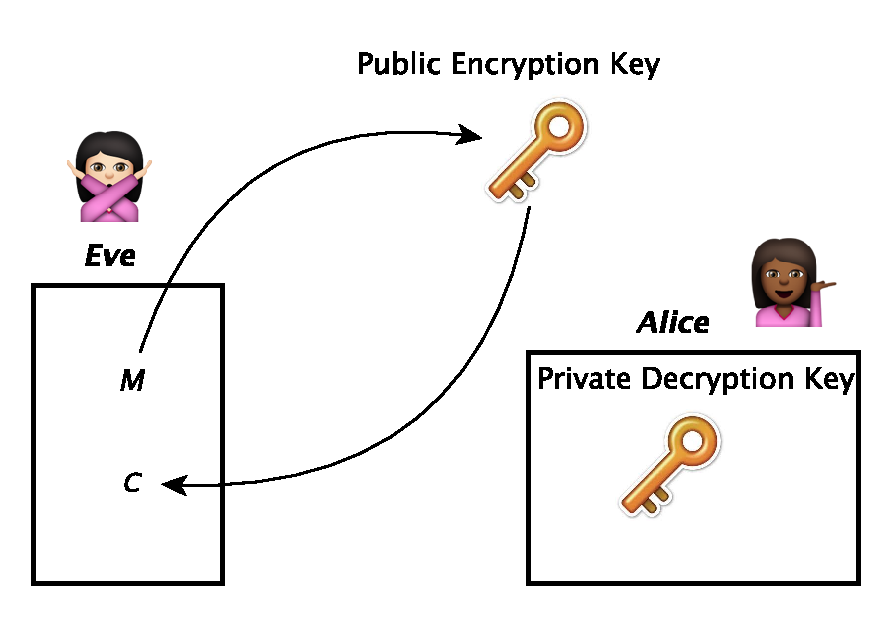
\includegraphics[scale=.5]{IMG/KPAattack.pdf}
\end{figure}\tiny
For instance, Alice may have a public key which any person can use to encrypt and send a message -- which only she is able to decrypt using the private key. In this case, Eve and encrypt any plaintext and view its ciphertext.
\end{frame}


\begin{frame}
\frametitle{Chosen-Ciphertext Model}

This should really be called a \emph{chosen-ciphertext-and-plaintext} model but that is too long. In this model, Eve can choose both plaintext values to encrypt as well as ciphertext values to decrypt.\newline

This is a very powerful form of security. 
\end{frame}

\begin{frame}
\frametitle{Chosen-Ciphertext Model}

\begin{itemize}
\item \emph{Given:} Plaintext messages and their corresponding encryptions; ciphertext messages and their corresponding decryptions 
\item \emph{Deduce:} $K$, the decryption key
\end{itemize}

Eve can choose any ciphertexts to be decrypted, and is able to access their decrypted plaintexts. 
\end{frame}


\begin{frame}
\frametitle{Chosen-Ciphertext Model: Black Box Decryption}

Eve is given what is called \textbf{black-box access} to a \textbf{Decryption Oracle}. She does not know the decryption key, but she is able to send ciphertexts of her choosing through this oracle and receive the corresponding plaintexts in return. 
\begin{figure}
\centering
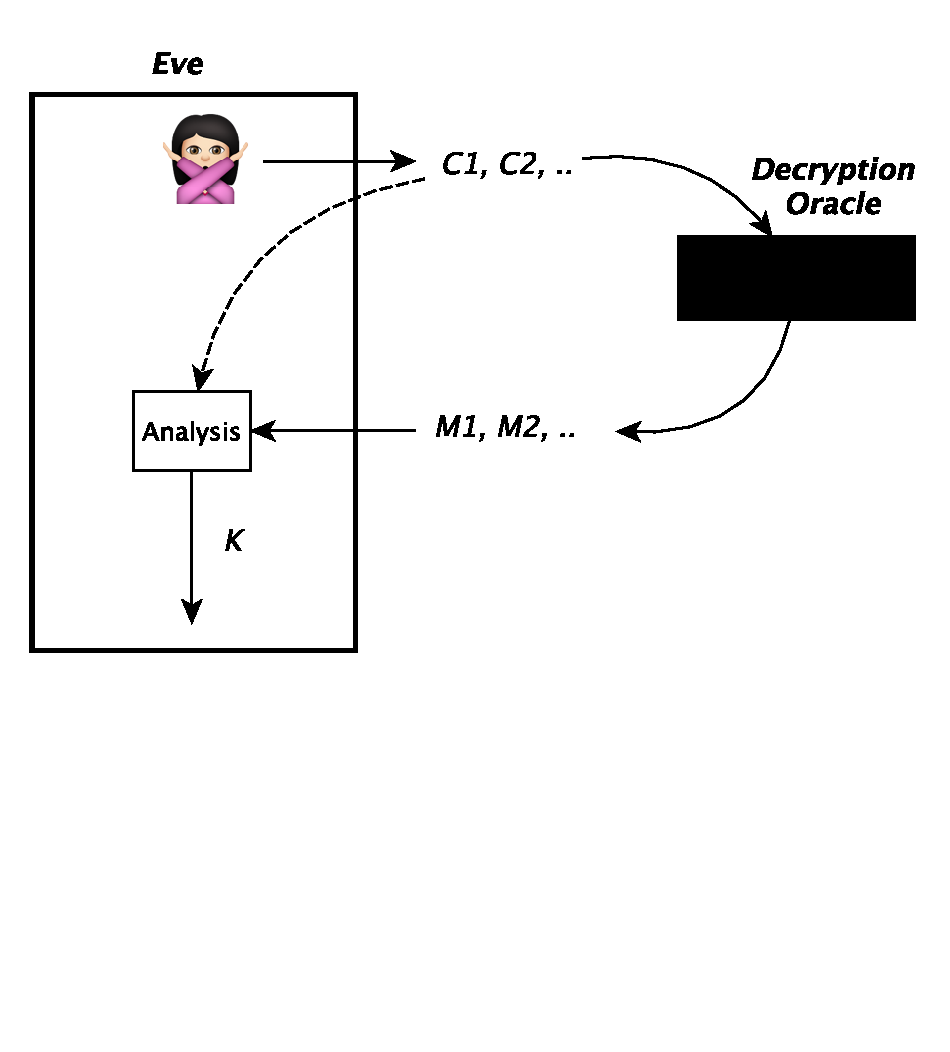
\includegraphics[scale=.5]{IMG/attack4.pdf}
\end{figure}
\end{frame}


\begin{frame}
\frametitle{Chosen-Ciphertext Model: The Game}

This is the \emph{offline} version, where Eve must choose all plaintext and ciphertext messages in advance. 
\begin{enumerate}
\item Eve chooses $M_1,\dots, M_n$ and $\hat C_1,\dots,\hat C_k$. 
\item Eve is given $C_i = D_K(M_i)$ for $1\le i\le n$ and $\hat M_j = E_{\hat k} (\hat C_j)$ for $1 \le j \le k$.
\item Eve deduces $K$, the decryption key. 
\end{enumerate}
\end{frame}

\begin{frame}
\frametitle{Adaptive Chosen-Ciphertext Model}

There is also a corresponding \emph{adaptive}, or \emph{online}, chosen-ciphertext model. In this case, Eve chooses a plaintext or ciphertext message, receives either its encryption or decryption, and can use this information to selectively pick her next plaintext or ciphertext. \newline

This is an even stronger model of security.
\end{frame}


\section{Attacks}

\begin{frame}
\frametitle{Other Attack Models}

The attacks described above attempt to recover the decryption key or the plaintext. However, it is possible to mount a different type of attack. Attacks could be designed to:
\begin{itemize}
\item Recover partial information about a plaintext (length, partial decryptions, etc)
\item Forge a message
\item Many many more!
\end{itemize}
\end{frame}

\begin{frame}
\frametitle{Distinguishing Attacks}

A \textbf{distinguishing attack} finds a difference between an ideal encryption scheme, where no information could possibly leaked in any case ever, and the encryption scheme we are using. \newline

This covers all possible attacks including ones not yet discovered.
\newline

What is a perfect encryption scheme?
\end{frame}

\begin{frame}
\frametitle{Unconditional Security}

We call an algorithm unconditionally secure if no amount of time and/or computational power would be enough for any adversary to ever recover the plaintext. The only unconditionally secure cryptosystem is the \textbf{one-time pad} which we will see next week.\newline

The one-time pad is not a feasible cryptosystem for most applications, hence the need for other cryptosystems. 
\end{frame}

\begin{frame}
\frametitle{Security}

Because unconditional security is not feasible in the real world, we must instead create cryptosystems which are resistant to feasible real-world attacks. 
\end{frame}

\begin{frame}
\frametitle{Brute-Force Attacks}

All other cryptosystems could be broken by a ciphertext-only attack. The attacker would simply have to try every possible key until she found the correct one. This is called a \textbf{brute-force attack.}\newline

A cryptosystem is called \textbf{computationally secure} if it is unfeasible to break the system with current and foreseeable future computational resources.  \newline

This is not generally a very feasible attack on a cryptosystem. Why not?
\end{frame}

\begin{frame}
\frametitle{Other Attacks}

\begin{itemize}
\item The attacker can base attacks based on how fast encryption and decryption operations take -- known as \textbf{timing attacks}.
\item An attack which uses this sort of additional leakage of information is called a \textbf{side-channel attack}.
\end{itemize}
\end{frame}

\begin{frame}
\frametitle{The Birthday Paradox}

The next attack we look at, called a \textbf{birthday attack}, is named after the \textbf{birthday paradox}.\newline

How many people do you need in a room before there is a $50\%$ chance that two of them share a birthday?
\end{frame}

\begin{frame}
\frametitle{The Birthday Paradox}

To calculate this, instead of calculating the probability of two people sharing a birthday we calculate the probability that a pair of people \emph{do not} share a birthday. \newline

The probability that two people have different birthdays is given by
\[
1 - \frac{1}{365} = \frac{364}{365} = .99726
\]
\end{frame}


\begin{frame}
\frametitle{The Birthday Paradox}

What is the probability that 4 people share a birthday? Well, given four people, there are ${4\choose 2 }= 6$ possible pairs of people. So the probability that every two out of four people have different birthday is given by 
\[
\left(\frac{364}{365}\right)^6 = 0.983\cdots
\]
\end{frame}

\begin{frame}
\frametitle{The Birthday Paradox}

Somewhat counterintuitively it only takes 23 people before the probability that all possible pairs of them do not share a birthday drops below $50\%$. Note that ${23 \choose 2} = 253$ and 
\[
\left(\frac{364}{365}\right)^{23} = 0.499\cdots
\]
So a slightly less than $50\%$ chance that any pair of people do \emph{not} share a birthday, which translates to slightly greater than $50\%$ chance that some pair of people share a birthday. 
\end{frame}


\begin{frame}
\frametitle{Birthday Attacks}

Birthday attacks use the fact that \textbf{collisions}, or duplicate values, occur more often than expected. 
\end{frame}

\begin{frame}
\frametitle{Example: Birthday Attacks}

Suppose there is a financial transaction system which uses a new $64$-bit key for each transaction. There are $2^{64}$ different keys, or over eighteen billion billion possible keys. After seeing only $2^{32}$ (four billion) transactions the attacker can expect that some pair of transactions likely used the same key. \newline

The attacker can use two messages with the same key  to forge a message which will still be authenticated, using its \textbf{message authentication code (MAC)}. This will be discussed further later in the course. 
\end{frame}

\begin{frame}
\frametitle{Birthday Attacks}

If an element can take $N$ values then we expect a collision after choosing approximately $\sqrt{N}$ random elements. \newline

When using encryption we often use bit-string representations of data. If there are $2^k$ possible bit strings of lenght $k$, then we need approximately $2^{k/2}$ elements before we can expect a collision. This is called the \textbf{birthday bound}.
\end{frame}



\begin{frame}
\frametitle{Meet-In-The-Middle Attacks}

This is another type of a known-plaintext attack. Now, Eve will build her own table of keys. \newline

In the previous example of the $64$-bit financial transaction system, Eve carries out this attack by first choosing $2^{23}$ $64$-bit keys at random. She then computes the MAC on the ``Are you ready to receive the transaction?'' message that is sent at the beginning of each round. If the MAC appears in her table then it is highly likely that the authentication key for that transaction is the same one the attacker used to compute that table entry, so Eve can recover this key. \newline

We will discuss this attack further later in the course. 
\end{frame}


\begin{frame}
\frametitle{Man-in-the-Middle Attacks}

These are a very common and useful form of attack. Eve now will insert herself in the middle of the conversation between Bob and Alice, and impersonate both of them in order to gain access to information they were trying to send each other.  \newline

We will discuss this in more detail later in the course.
\end{frame}

\begin{frame}
\frametitle{References}

These slides are based off of Sections 2.6 and 2.7 of \emph{Cryptography Engineering} by Ferguson, Schneier, and Kohno.
\end{frame}
\end{document}


